\section{Proposed methods}
\label{sec:methods}

In general, there are two approaches to solve this problem,
\begin{enumerate}
\item \emph{Scoring POIs}, and then pick the $K-1$ highest scored POIs from $\mathcal{P} \setminus s$,
\item \emph{Scoring trajectories}, and then pick the highest scored trajectory with respect to query $\mathbf{x}$.
\end{enumerate}

In this section, we briefly describe a variety of methods that following these two approaches.
Suppose the training set contains $N$ trajectories 
$\{ \mathbf{x}^{(i)}, \mathbf{y}^{(i)} \}_{i=1}^N$,
where $\mathbf{y}^{(i)}$ is the $i$-th trajectory and $\mathbf{x}^{(i)} = (y_1^{(i)},~ \mid\!\! \mathbf{y}^{(i)} \!\!\mid)$ is the query 
with respect to trajectory $\mathbf{y}^{(i)}$.



\subsection{Scoring POIs}
\label{sec:scoring_point}

We have a POI scoring function $S: \mathcal{X} \to \mathbb{R}^{\mid \mathcal{P} \mid}$, 
and the target trajectory is produced by sorting all POIs in descending order according to their scores 
$S(p \mid \mathbf{x}),~ \forall p \in \mathcal{P}$,
then picking the top $K-1$ from $\mathcal{P} \setminus s$.

First, we construct POI feature vectors $\Psi$ and labels $R$ for trajectories in training set, 
\begin{align*}
\Psi &= \left( \Psi(\mathbf{x}^{(i)}, p) \right)_{i=1,\dots,N,~p \in \mathcal{P}} = \left( \Psi_p^i \right)_{i,p}
        \in \mathbb{R}^{(N \cdot \mid \mathcal{P} \mid) \times D}, \\
   R &= \left( r(\mathbf{y}^{(i)}, p) \right)_{i=1,\dots,N,~p \in \mathcal{P}} = \left(r_p^i \right)_{i,p}
        \in \mathbb{R}^{(N \cdot \mid \mathcal{P} \mid) \times 1},
\end{align*}
where $D$ is the dimension of feature vector and label $r(\mathbf{y}, p)$ is computed from the location of POI $p$ in trajectory $\mathbf{y}$,
\begin{equation*}
r(\mathbf{y}, p) = \frac{1}{\mid\!\! \mathcal{P} \!\!\mid} 
                   \sum_{j=1}^{\mid \mathbf{y} \mid} (\mid\!\! \mathcal{P} \!\!\mid\! - j + 1) \cdot \llb y_j = p \rrb,
\end{equation*}
here $\llb \cdot \rrb$ is the indicator function, and the $j$-th POI in $\mathbf{y}$ will be scored $\mid\!\! \mathcal{P} \!\!\mid\! - j + 1$, 
any POI that does not appear in $\mathbf{y}$ will be scored $0$ ($0$ is an arbitrary choice).



\subsubsection{Occurrence prediction}
\label{sec:logistic}

To begin with, we can simply ignore the order of POIs in a trajectory and just model the occurrence of a POI.
Formally, we construct binary labels
\begin{equation*}
l_p^i = \begin{cases}
+1,~p \in \mathbf{y}^{(i)} \\
-1,~p \notin \mathbf{y}^{(i)}
\end{cases}
\hspace{-1em}
= \begin{cases}
+1,~ r_p^i > 0 \\
-1,~ r_p^i = 0
\end{cases}
\end{equation*}
and train a logistic regression model 
%\begin{flalign*} % full-length alignment (align left), note the double-& at the end of equation
%\textsc{\underline{objective}} \hspace{2em} 
\begin{equation*}
\min_{\mathbf{w}} \frac{1}{2} \mathbf{w}^\top \mathbf{w} + 
%C \sum_{i=1}^N \sum_{p \in \mathcal{P}} \log \left(1 + \exp (- l_p^i \cdot \mathbf{w}_p^\top \Psi_p^i) \right), %&&
C \sum_{i=1}^N \sum_{p \in \mathcal{P}} \phi \left( l_p^i \cdot \mathbf{w}_p^\top \Psi_p^i) \right), %&&
\end{equation*}
%\end{flalign*}
where $\phi(z) = \log(1+\exp(-z))$ is a loss function, $\mathbf{w}$ is an ensemble of all POI specific parameters $\mathbf{w}_p, p \in \mathcal{P}$,
and $C>0$ is a regularisation constant.
We can also share parameters between POIs by assuming $\mathbf{w}_p = \mathbf{u} + \mathbf{v}_p$.

The score of POI $p$ is the probability of $p$ occurring in trajectory $\mathbf{y}$ given query $\mathbf{x}$
\begin{equation*}
S(p \mid \mathbf{x})
= \mathbb{P}(p \in \mathbf{y} \mid \mathbf{x}; \mathbf{w})
= \mathbb{P}(r(\mathbf{y}, p) > 0 \mid \mathbf{x}; \mathbf{w})
= \sigma \left( \mathbf{w}_p^\top \Psi(\mathbf{x}, p) \right),
\end{equation*}
where $\sigma(z) = \frac{1}{1+\exp({-z})}$ is the logistic function.



\subsubsection{POI scoring for each location}
\label{sec:multi}

Furthermore, we can model the probability of POI $p$ at location $k$ given query $\mathbf{x}$.
That is, for each query $\mathbf{x}^{(i)},~ \forall i$, 
we train a $\mid\!\! \mathcal{P} \!\!\mid$-class $K$-label classifier with examples $\{ \mathbf{x}^{(i)}, y_k^{(i)} \}_{k=2}^K$
using the one-versus-rest approach,
\begin{equation*}
\mathbb{P}(y_k = p \mid \mathbf{x}) = \frac{\exp \left( \mathbf{w}^\top \Psi(\mathbf{x}, p, k) \right)}
                                           {\sum_{p' \in \mathcal{P}} \exp \left( \mathbf{w}^\top \Psi(\mathbf{x}, p', k) \right)}.
\end{equation*}

The recommendation is simply done by picking the most likely POI for each location $k$ independently,
\begin{equation*}
y_k^* = \argmax_{p \in \mathcal{P}}~ \mathbb{P}(y_k = p \mid \mathbf{x}),~ k = 2, \dots, K.
\end{equation*}

This approach can be described by a directed graphical model as shown in Figure~\ref{fig:pgm}(a).



\subsubsection{Direct rank prediction}
\label{sec:linear}

On the other hand, we can directly model the location/rank of a POI in a trajectory.
Formally, we train a linear regression model to minimise the empirical squared loss (with L2 regularisation)
\begin{equation*}
\min_{\mathbf{w}} \frac{1}{2} \mathbf{w}^\top \mathbf{w} + C \sum_{i=1}^N \sum_{p \in \mathcal{P}} \|r_p^i - \hat{r}_p^i \|^2, 
\end{equation*}
where the predicted rank $\hat{r}_p^i = \mathbf{w}_p^\top \Psi_p^i$, 
and parameter settings are similar to those described in Section~\ref{sec:logistic},
and examples with $0$ labels, i.e., $r_p^i = 0$ are ignored in training.

The score of POI $p$ is the expected rank of $p$ given query $\mathbf{x}$ 
\begin{equation*}
S(p \mid \mathbf{x})
= \mathbb{E}(\hat{r}_p \mid \mathbf{x}; \mathbf{w}) 
= \mathbf{w}_p^\top \Psi(\mathbf{x}, p).
\end{equation*}

%To learn the parameters $\mathbf{w}$, we need to solve linear equations $\Psi \cdot \mathbf{w} = R$,
%which is straightforward, i.e., $\mathbf{w} = \Psi^{-1} R$ or $\mathbf{w} = \Psi \backslash R$ by using matrix left division.

We note that when two different trajectories satisfy the same query, the feature vectors (Section~\ref{sec:feature}) for all POIs will be the same 
but the labels (i.e., ranks) can be different, which may confuse this model. In this case, the prediction (by this model) will be the average rank.




\subsubsection{Pairwise ranking}
\label{sec:rank}

Let $\phi(\cdot)$ be a loss function and $l_{p,p'}^i$ be a binary label
\begin{equation*}
l_{p,p'}^i = \begin{cases}
+1,~ \mathbf{y}^{(i)} ~\text{prefers}~ p, \\
-1,~ \mathbf{y}^{(i)} ~\text{prefers}~ p'.
\end{cases}
\end{equation*}
We can learn a ranking model
\begin{equation*}
\min_{\mathbf{w}} \frac{1}{2} \mathbf{w}^\top \mathbf{w} +  
C \sum_{i=1}^N \sum_{p, p' \in \mathcal{P}} \phi \left( l_{p,p'}^i \cdot \mathbf{w}^\top (\Psi_p^i - \Psi_{p'}^i) \right).
\end{equation*}

There are a number of options for the design of labels $l_{p,p'}^i$,
\begin{itemize}
\item let $c_p^i$ denotes the number of times POI $p$ was observed in trajectories satisfying query $\mathbf{x}^{(i)}$ (except the start POI), and define
      \begin{equation*}
      l_{p,p'}^i = \begin{cases}
      +1,~ c_p^i > c_{p'}^i, \\
      -1,~ c_p^i < c_{p'}^i.
      \end{cases}
      \end{equation*}
      This definition reflects whether $p$ was occurred more frequently than $p'$ for query $\mathbf{x}^{(i)}$.
      To deal with ties, i.e., $\{(p, p') \mid c_p^i = c_{p'}^i\}$, we generate both the positive and the negative labels for these examples.
\item Alternatively, we can define
      \begin{equation*}
      l_{p,p'}^i = \begin{cases}
      +1,~ r(\mathbf{y}^{(i)}, p) > r(\mathbf{y}^{(i)}, p'), \\
      -1,~ r(\mathbf{y}^{(i)}, p) < r(\mathbf{y}^{(i)}, p').
      \end{cases}
      \end{equation*}
      There will be no ties when $p \ne p'$ and $p, p' \in \mathbf{y}^{(i)}$, if we remove examples that $r_p^i = 0$.
\end{itemize}


Similarly, we have a few options for the design of loss function $\phi(\cdot)$,
\begin{itemize}
\item if $\phi(z) = \max(0,~ 1-z)^2$, we are training a rankSVM with linear kernel and L2 loss, and the ranking score 
      \begin{equation*}
      S(p \mid \mathbf{x})= \mathbf{w}^\top \Psi(\mathbf{x}, p);
      \end{equation*}
\item if $\phi(z) = \log(1 + \exp(-z))$, we are training a logistic regression model, and the ranking score
      \begin{equation*}
      S(p \mid \mathbf{x})= \mathbb{P}(p \mid \mathbf{x}; \mathbf{w}) = \sigma \left(\mathbf{w}^\top \Psi(\mathbf{x}, p) \right).
      \end{equation*}
      We can train this ranking model by gradient descent. Let $J(\mathbf{w})$ be the cost function we want to minimise, i.e.,
      \begin{align*}
      J(\mathbf{w})
      &= \frac{1}{2} \mathbf{w}^\top \mathbf{w} +  
         C \sum_{i=1}^N \sum_{p, p' \in \mathcal{P}} \phi \left( l_{p,p'}^i \cdot \mathbf{w}^\top (\Psi_p^i - \Psi_{p'}^i) \right) \\
      &= \frac{1}{2} \mathbf{w}^\top \mathbf{w} + 
         C \sum_{i=1}^N \sum_{p, p' \in \mathcal{P}} \log\left(1 + \exp\left(-l_{p,p'}^i \cdot \mathbf{w}^\top (\Psi_p^i - \Psi_{p'}^i) \right)\right).
      \end{align*}
      The gradient of the cost function w.r.t. parameters $\mathbf{w}$ is
      \begin{align*}
      \frac{\partial J(\mathbf{w})}{\partial \mathbf{w}} 
      &= \mathbf{w} + C \sum_{i=1}^N \sum_{p, p' \in \mathcal{P}} 
         \frac{-l_{p,p'}^i \cdot (\Psi_p^i - \Psi_{p'}^i) \cdot \exp\left( -l_{p,p'}^i \cdot \mathbf{w}^\top (\Psi_p^i - \Psi_{p'}^i) \right)}
              {1 + \exp\left( -l_{p,p'}^i \cdot \mathbf{w}^\top (\Psi_p^i - \Psi_{p'}^i) \right)} \\
      &= \mathbf{w} + C \sum_{i=1}^N \sum_{p, p' \in \mathcal{P}} 
         \frac{-l_{p,p'}^i \cdot (\Psi_p^i - \Psi_{p'}^i)}{1 + \exp\left( l_{p,p'}^i \cdot \mathbf{w}^\top (\Psi_p^i - \Psi_{p'}^i) \right)}.
      \end{align*} 
\end{itemize}

      
Compared with the first definition, the second option can implicitly incorporate the rank of a POI into the binary labels.



\subsubsection{Discussion}

We note that the point-wise POI scoring approaches (Section~\ref{sec:logistic} to \ref{sec:linear}) do not consider the inter-dependencies between POIs,
and the pairwise ranking approach (Section~\ref{sec:rank}) only considers the relative order between two individual points,
i.e., modelling each pair independently.



\subsection{Scoring trajectories}
\label{sec:structured}

One approach that captures long-term dependencies is scoring a trajectory as a whole,
that is, we model the dependences between different POIs in a trajectory by employing structured prediction models,
e.g., probabilistic models such as maximum-entropy Markov models (MEMM) and conditional random fields (CRF),
or non-probabilistic model such as structured SVM.

We model the desired trajectory with respect to query $\mathbf{x}$ as a sequence of discrete variables with inter-dependencies,
each variable has $|\mathcal{P}|$ states, and the first variable being observed.
To make a recommendation, we find a trajectory that achieves the highest score
\begin{equation*}
\mathbf{y}^* = \argmax_{\mathbf{y} \in \mathcal{Y}_\mathbf{x}}~ f(\mathbf{x}, \mathbf{y}),
\end{equation*}
%where $\mathcal{Y}_\mathbf{x}$ is the set of all possible trajectories with POIs in $\mathcal{P}$ and satisfying query $\mathbf{x}$,
where $f(\mathbf{x}, \mathbf{y})$ is a function that scores the compatibility between query $\mathbf{x}$ and a specific trajectory $\mathbf{y}$,
and different models described in this section basically employ different formulations of $f(\cdot,\cdot)$. % with respect to different assumptions.


\begin{figure}[t]
    \centering
    \begin{subfigure}[t]{.33\textwidth} % textwidth in figure environment
        \centering
        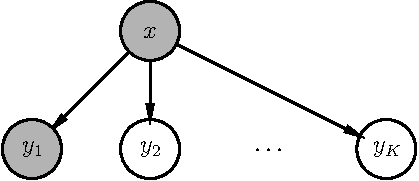
\includegraphics[width=.8\textwidth]{mmclassifier.pdf} % textwidth in subfigure environment
        \caption{Multi-class multi-label classifier}
    \end{subfigure}
    \begin{subfigure}[t]{.33\textwidth}
        \centering
        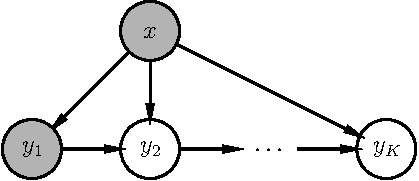
\includegraphics[width=.8\textwidth]{memm.pdf}
        \caption{MEMM}
    \end{subfigure}
    \begin{subfigure}[t]{.33\textwidth}
        \centering
        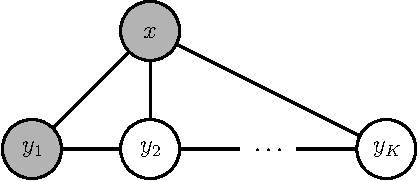
\includegraphics[width=.8\textwidth]{crf.pdf}
        \caption{CRF}
    \end{subfigure}
    \caption{Graphical models for trajectory recommendation.}
    \label{fig:pgm}
\end{figure}


\subsubsection{Maximum-entropy Markov models}
\label{sec:memm}

For MEMM, the compatibility function $f(\mathbf{x}, \mathbf{y})$ is the probability of trajectory $\mathbf{y}$ given query $\mathbf{x} = (s, K)$,
\begin{equation*}
f(\mathbf{x}, \mathbf{y}) 
= \mathbb{P}(\mathbf{y} \mid \mathbf{x}; \mathbf{w}) 
= \mathbb{P}(y_1 \mid \mathbf{x}; \mathbf{w}) \cdot \prod_{j=2}^K \mathbb{P}(y_j \mid y_{j-1}, \mathbf{x}; \mathbf{w})
= 1 \cdot \prod_{j=2}^{K}~
  \frac{\exp \left(\mathbf{w}^\top \Psi_j(\mathbf{x}, y_{j-1}, y_j) \right)}
       {\sum_{y' \in \mathcal{P}} \exp \left(\mathbf{w}^\top \Psi_j(\mathbf{x}, y_{j-1}, y') \right)},
\end{equation*}
where we do local normalisation.

The negative log-likelihood of training set is
\begin{equation*}
\ell(\mathbf{w}) 
= -\sum_{i=1}^N \log \mathbb{P}(\mathbf{y}^{(i)} \mid \mathbf{x}^{(i)}; \mathbf{w}) \\
= -\sum_{i=1}^N \sum_{j=2}^{\mid \mathbf{y}^{(i)} \mid} 
                \mathbf{w}^\top \Psi_j(\mathbf{x}^{(i)}, y_{j-1}^{(i)}, y_j^{(i)}) +
   \sum_{i=1}^N \sum_{j=2}^{\mid \mathbf{y}^{(i)} \mid} 
                \log \sum_{y' \in \mathcal{P}} \exp \left(\mathbf{w}^\top \Psi_j(\mathbf{x}^{(i)}, y_{j-1}^{(i)}, y') \right).
\end{equation*}

To learn the parameters, we maximise the likelihood of training set by minimising its negative log-likelihood (with L2 regularisation)
\begin{equation}
\label{eq:trainmemm}
\min_{\mathbf{w}} \frac{1}{2} \mathbf{w}^\top \mathbf{w} + C \ell(\mathbf{w}).
\end{equation}

A straightforward approach to optimise the above objective is employing gradient descent. 
Let $J(\mathbf{w})$ be the objective (cost function), i.e.,
\begin{align*}
J(\mathbf{w}) 
&= \frac{1}{2} \mathbf{w}^\top \mathbf{w} + C \ell(\mathbf{w}) \\
&= \frac{1}{2} \mathbf{w}^\top \mathbf{w} -
   C \sum_{i=1}^N \sum_{j=2}^{\mid \mathbf{y}^{(i)} \mid} \mathbf{w}^\top \Psi_j(\mathbf{x}^{(i)}, y_{j-1}^{(i)}, y_j^{(i)}) +
   C \sum_{i=1}^N \sum_{j=2}^{\mid \mathbf{y}^{(i)} \mid} \log \sum_{y' \in \mathcal{P}} 
     \exp \left(\mathbf{w}^\top \Psi_j(\mathbf{x}^{(i)}, y_{j-1}^{(i)}, y') \right).
\end{align*}
The gradient of the cost function w.r.t. parameters $\mathbf{w}$ is
\begin{align*}
\frac{\partial J{\mathbf{w}}}{\partial \mathbf{w}}
&= \mathbf{w} + C \frac{\partial \ell(\mathbf{w})}{\partial \mathbf{w}} \\
&= \mathbf{w} - C \sum_{i=1}^N \sum_{j=2}^{\mid \mathbf{y}^{(i)} \mid} \Psi_j(\mathbf{x}^{(i)}, y_{j-1}^{(i)}, y_j^{(i)}) +
   C \sum_{i=1}^N \sum_{j=2}^{\mid \mathbf{y}^{(i)} \mid} 
     \frac{\sum_{y' \in \mathcal{P}} \left( \Psi_j(\mathbf{x}^{(i)}, y_{j-1}^{(i)}, y') \cdot 
           \exp \left(\mathbf{w}^\top \Psi_j(\mathbf{x}^{(i)}, y_{j-1}^{(i)}, y') \right) \right)}
          {\sum_{y' \in \mathcal{P}} \exp \left(\mathbf{w}^\top \Psi_j(\mathbf{x}^{(i)}, y_{j-1}^{(i)}, y') \right)}.
\end{align*}


MEMM is a directed graphical model (as shown in Figure~\ref{fig:pgm}(b)) which captures transitions from one POI to any other POIs simultaneously, 
in contrast, pairwise ranking (Section~\ref{sec:rank}) captures only pairwise relations independently.

To make a prediction, we need to do a MAP inference (which can be done using the Viterbi algorithm if duplicated POIs are permitted)
\begin{equation}
\label{eq:testmemm}
\begin{aligned}
\mathbf{y}^* 
&= \argmax_{\mathbf{y} \in \mathcal{Y}_\mathbf{x}}~f(\mathbf{x}, \mathbf{y})
 = \argmax_{\mathbf{y} \in \mathcal{Y}_\mathbf{x}}~\mathbb{P}(\mathbf{y} \mid \mathbf{x}; \mathbf{w})
 = \argmax_{\mathbf{y} \in \mathcal{Y}_\mathbf{x}}~\log \mathbb{P}(\mathbf{y} \mid \mathbf{x}; \mathbf{w}) \\
&= \argmax_{\mathbf{y} \in \mathcal{Y}_\mathbf{x}}~\sum_{j=2}^{K} \mathbf{w}^\top \Psi_j(\mathbf{x}, y_{j-1}, y_j) - 
   \sum_{j=2}^{K} \log \sum_{y' \in \mathcal{P}} \exp \left(\mathbf{w}^\top \Psi_j(\mathbf{x}, y_{j-1}, y') \right).
\end{aligned}
\end{equation}

Furthermore, we can explicitly model dependencies between POIs in trajectory by adding dependences between variable $y_j$ and $y_k,~ j < k$,
which results in another compatibility function
\begin{equation*}
f(\mathbf{x}, \mathbf{y}) 
= \mathbb{P}(\mathbf{y} \mid \mathbf{x}; \mathbf{w}) 
= \mathbb{P}(y_1 \mid \mathbf{x}; \mathbf{w}) \cdot \prod_{j=2}^K \mathbb{P}(y_j \mid y_1,\dots, y_{j-1}, \mathbf{x}; \mathbf{w})
= 1 \cdot \prod_{j=2}^{K}~
  \frac{\exp \left(\mathbf{w}_j^\top \Psi_j(\mathbf{x}, y_1, \dots, y_{j-1}, y_j) \right)}
       {\sum_{y' \in \mathcal{P}} \exp \left(\mathbf{w}_j^\top \Psi_j(\mathbf{x}, y_1, \dots, y_{j-1}, y') \right)}.
\end{equation*}

It can be trained similarly using the maximum likelihood principle.



\subsubsection{Conditional random fields}
\label{sec:crf}

For linear chain CRF, the compatibility function $f(\mathbf{x}, \mathbf{y})$ is also the probability of trajectory $\mathbf{y}$ given
query $\mathbf{x} = (s, K)$,
\begin{equation*}
f(\mathbf{x}, \mathbf{y}) = \mathbb{P}(\mathbf{y} \mid \mathbf{x}; \mathbf{w}) 
= \frac{\exp \left( \mathbf{w}^\top \Psi(\mathbf{x}, \mathbf{y}) \right)}
       {\sum_{\mathbf{y}' \in \mathcal{Y}_\mathbf{x}} \exp \left( \mathbf{w}^\top \Psi(\mathbf{x}, \mathbf{y}') \right)}
= \frac{\prod_{j=2}^{K} \exp \left( \mathbf{w}_j^\top \Psi_j(\mathbf{x}, y_{j-1}, y_j) \right)}
       {\sum_{\mathbf{y}' \in \mathcal{Y}_\mathbf{x}} \prod_{j=2}^{K} \exp \left( \mathbf{w}_j^\top \Psi_j(\mathbf{x}, y_{j-1}', y_j') \right)},
\end{equation*}
where $\mathbf{y} \in \mathcal{Y}_\mathbf{x}$ and we assume decomposition 
$\mathbf{w}^\top \Psi(\mathbf{x}, \mathbf{y}) = \sum_{j=2}^{K} \mathbf{w}_j^\top \Psi_j(\mathbf{x}, y_{j-1}, y_j)$.
The denominator is known as the \emph{partition function} and we do global normalisation.

The negative log-likelihood of training set is
\begin{equation*}
\ell(\mathbf{w}) 
= -\sum_{i=1}^N \log \mathbb{P}(\mathbf{y}^{(i)} \mid \mathbf{x}^{(i)}; \mathbf{w})
= -\sum_{i=1}^N \sum_{j=2}^{\mid \mathbf{y}^{(i)} \mid} \mathbf{w}_j^\top \Psi_j(\mathbf{x}^{(i)}, y_{j-1}^{(i)}, y_j^{(i)}) +
   \sum_{i=1}^N \log \sum_{\mathbf{y}' \in \mathcal{Y}_\mathbf{x}} 
                \prod_{j=2}^{K} \exp \left(\mathbf{w}_j^\top \Psi_j(\mathbf{x}^{(i)}, y_{j-1}', y_j')\right).
\end{equation*}

To learn the parameters, we maximise the likelihood of training set by minimising its negative log-likelihood (with L2 regularisation)
\begin{equation}
\label{eq:traincrf}
\min_{\mathbf{w}} \frac{1}{2} \mathbf{w}^\top \mathbf{w} + C \ell(\mathbf{w}).
\end{equation}

CRF is an undirected graphical model as shown in Figure~\ref{fig:pgm}(c).
Similar to MEMM, CRF can capture transitions from one POI to any other POIs simultaneously.
To make a prediction, we need to do a MAP inference
\begin{equation}
\label{eq:testcrf}
\begin{aligned}
\mathbf{y}^* 
&= \argmax_{\mathbf{y} \in \mathcal{Y}_\mathbf{x}}~f(\mathbf{x}, \mathbf{y})
 = \argmax_{\mathbf{y} \in \mathcal{Y}_\mathbf{x}}~\mathbb{P}(\mathbf{y} \mid \mathbf{x}; \mathbf{w})
 = \argmax_{\mathbf{y} \in \mathcal{Y}_\mathbf{x}}~\log \mathbb{P}(\mathbf{y} \mid \mathbf{x}; \mathbf{w}) \\
&= \argmax_{\mathbf{y} \in \mathcal{Y}_\mathbf{x}}~\sum_{j=2}^{K} \mathbf{w}_j^\top \Psi_j(\mathbf{x}, y_{j-1}, y_j) -
   \log \sum_{\mathbf{y}' \in \mathcal{Y}_\mathbf{x}} \prod_{j=2}^{K} \exp \left( \mathbf{w}_j^\top \Psi_j(\mathbf{x}, y_{j-1}', y_j') \right).
\end{aligned}
\end{equation}

\eat{TODO: why people usually employ CRF?}


\subsubsection{Structured SVM}
\label{sec:ssvm}

For structured SVM, the compatibility function $f(\mathbf{x}, \mathbf{y})$ is this linear form,
\begin{equation*}
f(\mathbf{x}, \mathbf{y}) = \mathbf{w}^\top \Psi(\mathbf{x}, \mathbf{y}),
\end{equation*}
where $\Psi(\mathbf{x}, \mathbf{y})$ is a \emph{joint feature map} 
that captures features extracted from both query $\mathbf{x}$ and trajectory $\mathbf{y}$.

The design of joint feature $\Psi(\cdot,\cdot)$ is problem specific, 
for trajectory recommendation, we assume decomposition
\begin{equation*}
\label{eq:jointfeature}
\mathbf{w}^\top \Psi(\mathbf{x}, \mathbf{y}) 
= \sum_{j=2}^{\mid \mathbf{y} \mid} 
  \left( \mathbf{w}_j^\top \Psi_j(\mathbf{x}, y_j) + 
  \mathbf{w}_{j-1,j}^\top \Psi_{j-1, j}(\mathbf{x}, y_{j-1}, y_j) \right),
\end{equation*}
where $\Psi_j$ is a feature vector of POI $y_j$ (w.r.t. query $\mathbf{x}$)
and $\Psi_{j-1,j}$ is a pairwise feature vector that captures the affinity of transition from POI $y_{j-1}$ to POI $y_j$.

To learn the parameters, we train the structured SVM by optimising a quadratic program (QP),
\begin{equation}
\label{eq:nslack}
\begin{aligned}
\min_{\mathbf{w}, ~\bm{\xi} \ge 0} ~& \frac{1}{2} \mathbf{w}^\top \mathbf{w} + \frac{C}{n} \sum_{i=1}^n \xi_i \\
s.t.~~ ~& \mathbf{w}^\top \Psi(\mathbf{x}^{(i)}, \mathbf{y}^{(i)}) - \mathbf{w}^\top \Psi(\mathbf{x}^{(i)}, \bar{\mathbf{y}}) \ge 
       \Delta(\mathbf{y}^{(i)}, \bar{\mathbf{y}}) - \xi_i, ~\bar{\mathbf{y}} \in \mathcal{Y}_{\mathbf{x}^{(i)}},~\forall i,
\end{aligned}
\end{equation}
where $\Delta(\mathbf{y}, \bar{\mathbf{y}})$ is a discrepancy function that measures the loss 
for predicting $\bar{\mathbf{y}}$ given ground truth $\mathbf{y}$, 
and slack variable $\xi_i$ is the \emph{hinge loss} for the prediction of the $i$-th example~\cite{tsochantaridis2005large},
\begin{equation*}
\xi_i = \max \left( 0,~ 
        \max_{\bar{\mathbf{y}} \in \mathcal{Y}_{\mathbf{x}^{(i)}}} 
        \left\{ \Delta(\mathbf{y}^{(i)}, \bar{\mathbf{y}}) + \mathbf{w}^\top \Psi(\mathbf{x}^{(i)}, \bar{\mathbf{y}}) \right\} -
        \mathbf{w}^\top \Psi(\mathbf{x}^{(i)}, \mathbf{y}^{(i)}) \right).
\end{equation*}
%This formulation is called "$n$-slack" as we have one slack variable for each example in training set.

We can rewrite the constraint in problem (\ref{eq:nslack}) as
\begin{equation}
\label{eq:ssvminf}
\mathbf{w}^\top \Psi(\mathbf{x}^{(i)}, \mathbf{y}^{(i)}) + \xi_i \ge
          \max_{\bar{\mathbf{y}} \in \mathcal{Y}_{\mathbf{x}^{(i)}}}
          \left\{\mathbf{w}^\top \Psi(\mathbf{x}^{(i)}, \bar{\mathbf{y}}) + \Delta(\mathbf{y}^{(i)}, \bar{\mathbf{y}}) \right\},~ \forall i,
\end{equation}
where the right hand side is known as the \emph{loss-augmented inference}.

To solve problem (\ref{eq:nslack}), one option is simply enumerating all constraints, and feeding the problem into a standard QP solver.
However, this approach is impractical as there is a constraint for every possible label $\bar{\mathbf{y}}$.
Instead, we use a cutting-plane algorithm which repeatedly solves QP (\ref{eq:nslack}) 
w.r.t. different set of constraints~\cite{joachims2009predicting}.
In each iteration, a new constraint is formed by solving the loss-augmented inference, 
which helps shrink the feasible region of the problem.



\subsubsection{Discussion}

All structured models described above suffer from a number of drawbacks.
\begin{enumerate}
\item The MEMM model (Section~\ref{sec:memm}) is relatively easy to train, 
      but the inference (Equation~\ref{eq:testmemm}) will not retain its efficiency if the no duplicates constraints are required.
\item The CRF model (Section~\ref{sec:crf}) suffers from inefficient training (Equation~\ref{eq:traincrf}) and 
      inference (Equation~\ref{eq:testcrf}) as the partition function cannot be computed efficiently.
\item Both the loss-augmented inference and prediction inference for structured SVM (Section~\ref{sec:ssvm}) cannot be done efficiently 
      if the no duplicates constraints are required.
\end{enumerate}

Approximate inference methods are critical for MEMM and CRF.
On the other hand, inference in structured SVM is equivalent to 
find a maximum-weight loop-less path with exactly $K$ edges in a complete weighted (both nodes and edges) graph, which is NP-hard (proof?).
Possible solutions including 
\begin{itemize}
\item formulating it as an integer linear program (ILP) and solve it using an ILP solver, 
      or using lazy constraint generation/cutting-plane techniques with a LP solver;
\item in addition, we can employ the list Viterbi algorithm~\cite{nilsson2001sequentially,seshadri1994list} 
      which sequentially find the next best (scored) trajectory until a maximum-weight loop-less path with exactly $K$ edges is found;
\item moreover, we can employ heuristics such as greedy search or the Christofides algorithm~\cite{christofides1976} 
      when the problem has the triangle inequality property (for trajectories, indeed).
\end{itemize}
These options are applicable to MEMM (Section~\ref{sec:memm}) as well.



\subsubsection{Inference algorithms}
\label{sec:inference}

\paragraph{Integer linear program}
If we formulate an ILP to do inference and employ the sub-tour elimination constraints from TSP, we have
\begin{alignat}{5}
& \max_{u,v} ~&& \sum_{k=1}^M \mathbf{w}_k^\top \phi_k(\mathbf{x}, p_k) \sum_{j=1}^M u_{jk} + 
                 \sum_{j=1}^M \sum_{k=1}^M u_{jk} \mathbf{w}_{jk}^\top \phi_{j, k}(\mathbf{x}, p_j, p_k) \\
& s.t. ~~ ~&& u_{jk}, ~z_j \in \{0, 1\}, ~u_{jj}=0, ~z_1=0, ~v_j \in \mathbf{Z},~ p_j \in \mathcal{P}, ~\forall j, k = 1,\cdots,M   \label{eq:cons1} \\
&          && \sum_{k=2}^M u_{1k} = 1, ~\sum_{j=2}^M u_{j1} = 0  \label{eq:cons2} \\
&          && \sum_{j=1}^M u_{jl} = z_l + \sum_{k=2}^M u_{lk} \le 1,   ~\forall l=2,\cdots,M                    \label{eq:cons3} \\
&          && \sum_{j=1}^M \sum_{k=1}^M u_{jk} = L-1,                                                           \label{eq:cons4} \\
&          && v_j - v_k + 1 \le (M-1) (1-u_{jk}),                     \forall j,k=2,\cdots,M                    \label{eq:cons5}
\end{alignat}
where $u_{jk}$ is a binary decision variable that determines whether the transition from $p_j$ to $p_k$ is in the resulting trajectory,
$z_j$ is a binary decision variable that determines whether $p_j$ is the last POI in trajectory.
$L$ is the number of POIs in trajectory.
For brevity, we arrange the POIs such that $p_1 = s$.
Firstly, the desired trajectory should start from $s$ (Constraint~\ref{eq:cons2}).
In addition, any POI could be visited at most once (Constraint~\ref{eq:cons3}).
Moreover, only $L-1$ transitions between POIs are permitted (Constraint~\ref{eq:cons4}),
i.e., the number of POI visits should be exactly $L$ (including $s$).
The last constraint, where $v_i$ is an auxiliary variable,
enforces that only a single sequence of POIs without sub-tours is permitted in the trajectory.

If we employ the above ILP to do loss-augmented inference, we can simply add a linear loss function to the objective, 
e.g., $\Delta(\mathbf{y}, \bar{\mathbf{y}}) = 1 - \sum_{j=1}^M \sum_{k=1}^M u_{j, y_k}$ if we define the loss as the number of mispredicted POIs,
where $\mathbf{y}$ is the ground truth and $\bar{\mathbf{y}}$ is the trajectory corresponding to the optimal solution of this ILP.

\paragraph{The list Viterbi algorithm}
Instead of employ an algorithm with exponential time complexity (e.g., ILP) to do inference,
we can resort to an iterative algorithm such as the list Viterbi algorithm~\cite{nilsson2001sequentially,seshadri1994list}
which sequentially find the $k$-th best (scored) trajectory given the best, $2$nd best, \dots, $(k-1)$-th best (scored) trajectories,
as described in Algorithm~\ref{alg:listviterbi}.


\begin{algorithm}[htbp]
\caption{The list Viterbi algorithm for inference}
\label{alg:listviterbi}
\begin{algorithmic}[1]
\STATE \textbf{Input}: $\mathbf{x}=(s, K),~ \mathcal{P},~ \mathbf{w},~ \Psi$
%\STATE Initialise score matrices $\alpha,~ \beta,~ f_t,~ f_{t, t+1}$, a max-heap $H,~ k=0$.
\STATE Initialise score matrices $\alpha,~ \beta,~ f_{t, t+1}$, a max-heap $H,~ k=0$.
\STATE $\triangleright$ Do the forward-backward procedure~\cite{rabiner1989tutorial}
\STATE $\forall p_j \in \mathcal{P},~ \alpha_t(p_j) = 
        \begin{cases}
        0,~ t = 1 \\
        \max_{p_i \in \mathcal{P}} \left\{ \alpha_{t-1}(p_i) + \mathbf{w}_{ij}^\top \Psi_{ij}(\mathbf{x}, p_i, p_j) + 
        \mathbf{w}_j^\top \Psi_j(\mathbf{x}, p_j) \right\},~ t=2,\dots,K
        \end{cases}$

\STATE $\forall p_i \in \mathcal{P},~ \beta_t(p_i) = 
        \begin{cases}
        0,~ t = K \\
        \max_{p_j \in \mathcal{P}} \left\{ \mathbf{w}_{ij}^\top \Psi_{ij}(\mathbf{x}, p_i, p_j) + 
        \mathbf{w}_j^\top \Psi_j(\mathbf{x}, p_j) + \beta_{t+1}(p_j) \right\},~ t = K-1,\dots,1
        \end{cases}$

%\STATE $\forall p_i \in \mathcal{P},~ f_t(p_i) = \alpha_t(p_i) + \beta_t(p_i),~ t = 1,\dots,K$
\STATE $\forall p_i, p_j \in \mathcal{P},~ f_{t,t+1}(p_i, p_j) = \alpha_t(p_i) + \mathbf{w}_{ij}^\top \Psi_{ij}(\mathbf{x}, p_i, p_j) + 
                              \mathbf{w}_j^\top \Psi_j(\mathbf{x}, p_j) + \beta_{t+1}(p_j),~ t = 1,\dots,K-1$

\STATE $\triangleright$ Identify the best (scored) trajectory $\mathbf{y}^1=(y_1^1,\dots,y_K^1)$ (possibly with sub-tours)
\STATE $y_t^1 = \begin{cases}
                s,~ t = 1 \\
%                \argmax_{p \in \mathcal{P}} \left\{ f_{1,2}(s, p) \right\},~ t = 2, \\
                \argmax_{p \in \mathcal{P}} \left\{ f_{t-1,t}(y_{t-1}^1, p) \right\},~ t = 2,\dots,K
                \end{cases}$

%\STATE $r^1 = \max_{p \in \mathcal{P}} \left\{ f_K(p) \right\}~~~ \triangleright$ $r^1$ is the score/priority of $\mathbf{y}^1$
\STATE $r^1 = \max_{p \in \mathcal{P}} \left\{ \alpha_{K}(p) \right\}~~~ \triangleright$ $r^1$ is the score/priority of $\mathbf{y}^1$
\STATE $H.\textit{push}\left(r^1,~ (\mathbf{y}^1, \textsc{nil}, \emptyset) \right)$

\WHILE{$H \ne \emptyset$ \textbf{and} $k < \,\mid\!\!\mathcal{P}\!\!\mid^{K-1} - \prod_{t=2}^K (\mid\!\!\mathcal{P}\!\!\mid-t+1)$}
    \STATE $r^k,~ (\mathbf{y}^k, I, S) = H.\textit{pop}()~~~ \triangleright$ 
           $r^k$ is the score of $\mathbf{y}^k=(y_1^k,\dots,y_K^k)$, $I$ is the partition index, and $S$ is the exclude set
    \STATE $k = k + 1$
    \RETURN $\mathbf{y}^k$ if NO sub-tours in $\mathbf{y}^k$
    \STATE $\bar{I} = \begin{cases}
                      2,~ I = \textsc{nil} \\
                      I,~ \text{otherwise}
                      \end{cases}$

    \FOR{$t = \bar{I},\dots,K$}
        \STATE $\bar{S} = \begin{cases}
                          S \cup \{ y_t^k \},~ t = \bar{I} \\
                          \{ y_t^k \},~ \text{otherwise}
                          \end{cases}$

        \STATE $\bar{y}_j = \begin{cases}
                            y_j^k,~~ j=1,\dots,t-1 \\
                            %\argmax_{p \in \mathcal{P} \setminus \textit{new\_exclude\_set}} f_{t-1,t}(y_{t-1}^k, p),~ j=t \\
                            \argmax_{p \in \mathcal{P} \setminus \bar{S}} \left\{ f_{t-1,t}(y_{t-1}^k, p) \right\},~ j=t \\
                            \argmax_{p \in \mathcal{P}} \left\{ f_{j-1, j}(\bar{y}_{j-1}, p) \right\},~ j=t+1,\dots,K
                \end{cases}$
        \STATE $\bar{r} = \begin{cases}
                          f_{t-1,t}(y_{t-1}^k, \bar{y}_t),~ I = \textsc{nil} \\
                          r^k + f_{t-1,t}(y_{t-1}^k, \bar{y}_t) - f_{t-1,t}(y_{t-1}^k, y_t^k),~ \text{otherwise}
                          \end{cases}$

        $H.\textit{push}\left(\bar{r}, (\bar{\mathbf{y}}, t, \bar{S}) \right)$
    \ENDFOR
\ENDWHILE
\end{algorithmic}
\end{algorithm}



\eat{
\subsection{Other models}
\label{sec:other}
Label ranking model,
Plackett-Luce probabilistic ranking
}


\section{Features}
\label{sec:feature}

\eat{
\underline{REVISE FEATURE DESIGN}
}

The POI and query specific features extracted from trajectories are shown in Table~\ref{tab:poifeature},
features that describe the transition preference between different POIs are shown in Table~\ref{tab:tranfeature}.



\begin{table*}[ht]
\caption{Features of POI $p$ with respect to query $(s,K)$}
\label{tab:poifeature}
\centering
\setlength{\tabcolsep}{10pt} % tweak the space between columns
\begin{tabular}{l|l} \hline
\textbf{Feature}  & \textbf{Description} \\ \hline
\texttt{category}               & one-hot encoding of the category of $p$ \\
\texttt{neighbourhood}          & one-hot encoding of the POI cluster that $p$ resides in \\
\texttt{popularity}             & logarithm of POI popularity of $p$ \\
\texttt{nVisit}                 & logarithm of the total number of visit by all users at $p$ \\
\texttt{avgDuration}            & logarithm of the average duration at $p$ \\ \hline

%\texttt{nOccurrence}            & the number of times $p$ occurred in a trajectory that satisfies the query \\ DON'T know given new query

\texttt{trajLen}                & trajectory length $K$, i.e., the number of POIs required \\
\texttt{sameCatStart}           & $1$ if the category of $p$ is the same as that of $s$, $-1$ otherwise \\
\texttt{sameNeighbourhoodStart} & $1$ if $p$ resides in the same POI cluster as $s$, $-1$ otherwise \\
\texttt{distStart}              & distance between $p$ and $s$, calculated using the Haversine formula \\
\texttt{diffPopStart}           & real-valued difference in POI popularity of $p$ from that of $s$ \\
\texttt{diffNVisitStart}        & real-valued difference in the total number of visit at $p$ from that at $s$ \\
\texttt{diffDurationStart}      & real-valued difference in average duration at $p$ from that at $s$ \\
\hline
\end{tabular}
\end{table*}



\begin{table}[ht]
\caption{POI features used to estimate the (feature-wise) transition probabilities}
\label{tab:tranfeature}
\centering
%\setlength{\tabcolsep}{28pt} % tweak the space between columns
\begin{tabular}{l|l} \hline
\textbf{Feature}       & \textbf{Description} \\ \hline
\texttt{category}      & category of POI \\
\texttt{neighbourhood} & the cluster that a POI resides in \\
\texttt{popularity}    & (discretised) popularity of POI \\
\texttt{nVisit}        & (discretised) total number of visit at POI \\
\texttt{avgDuration}   & (discretised) average duration at POI \\ \hline
\end{tabular}
\end{table}
